
%\begin{figure}[htbp]
%    \begin{center}
%    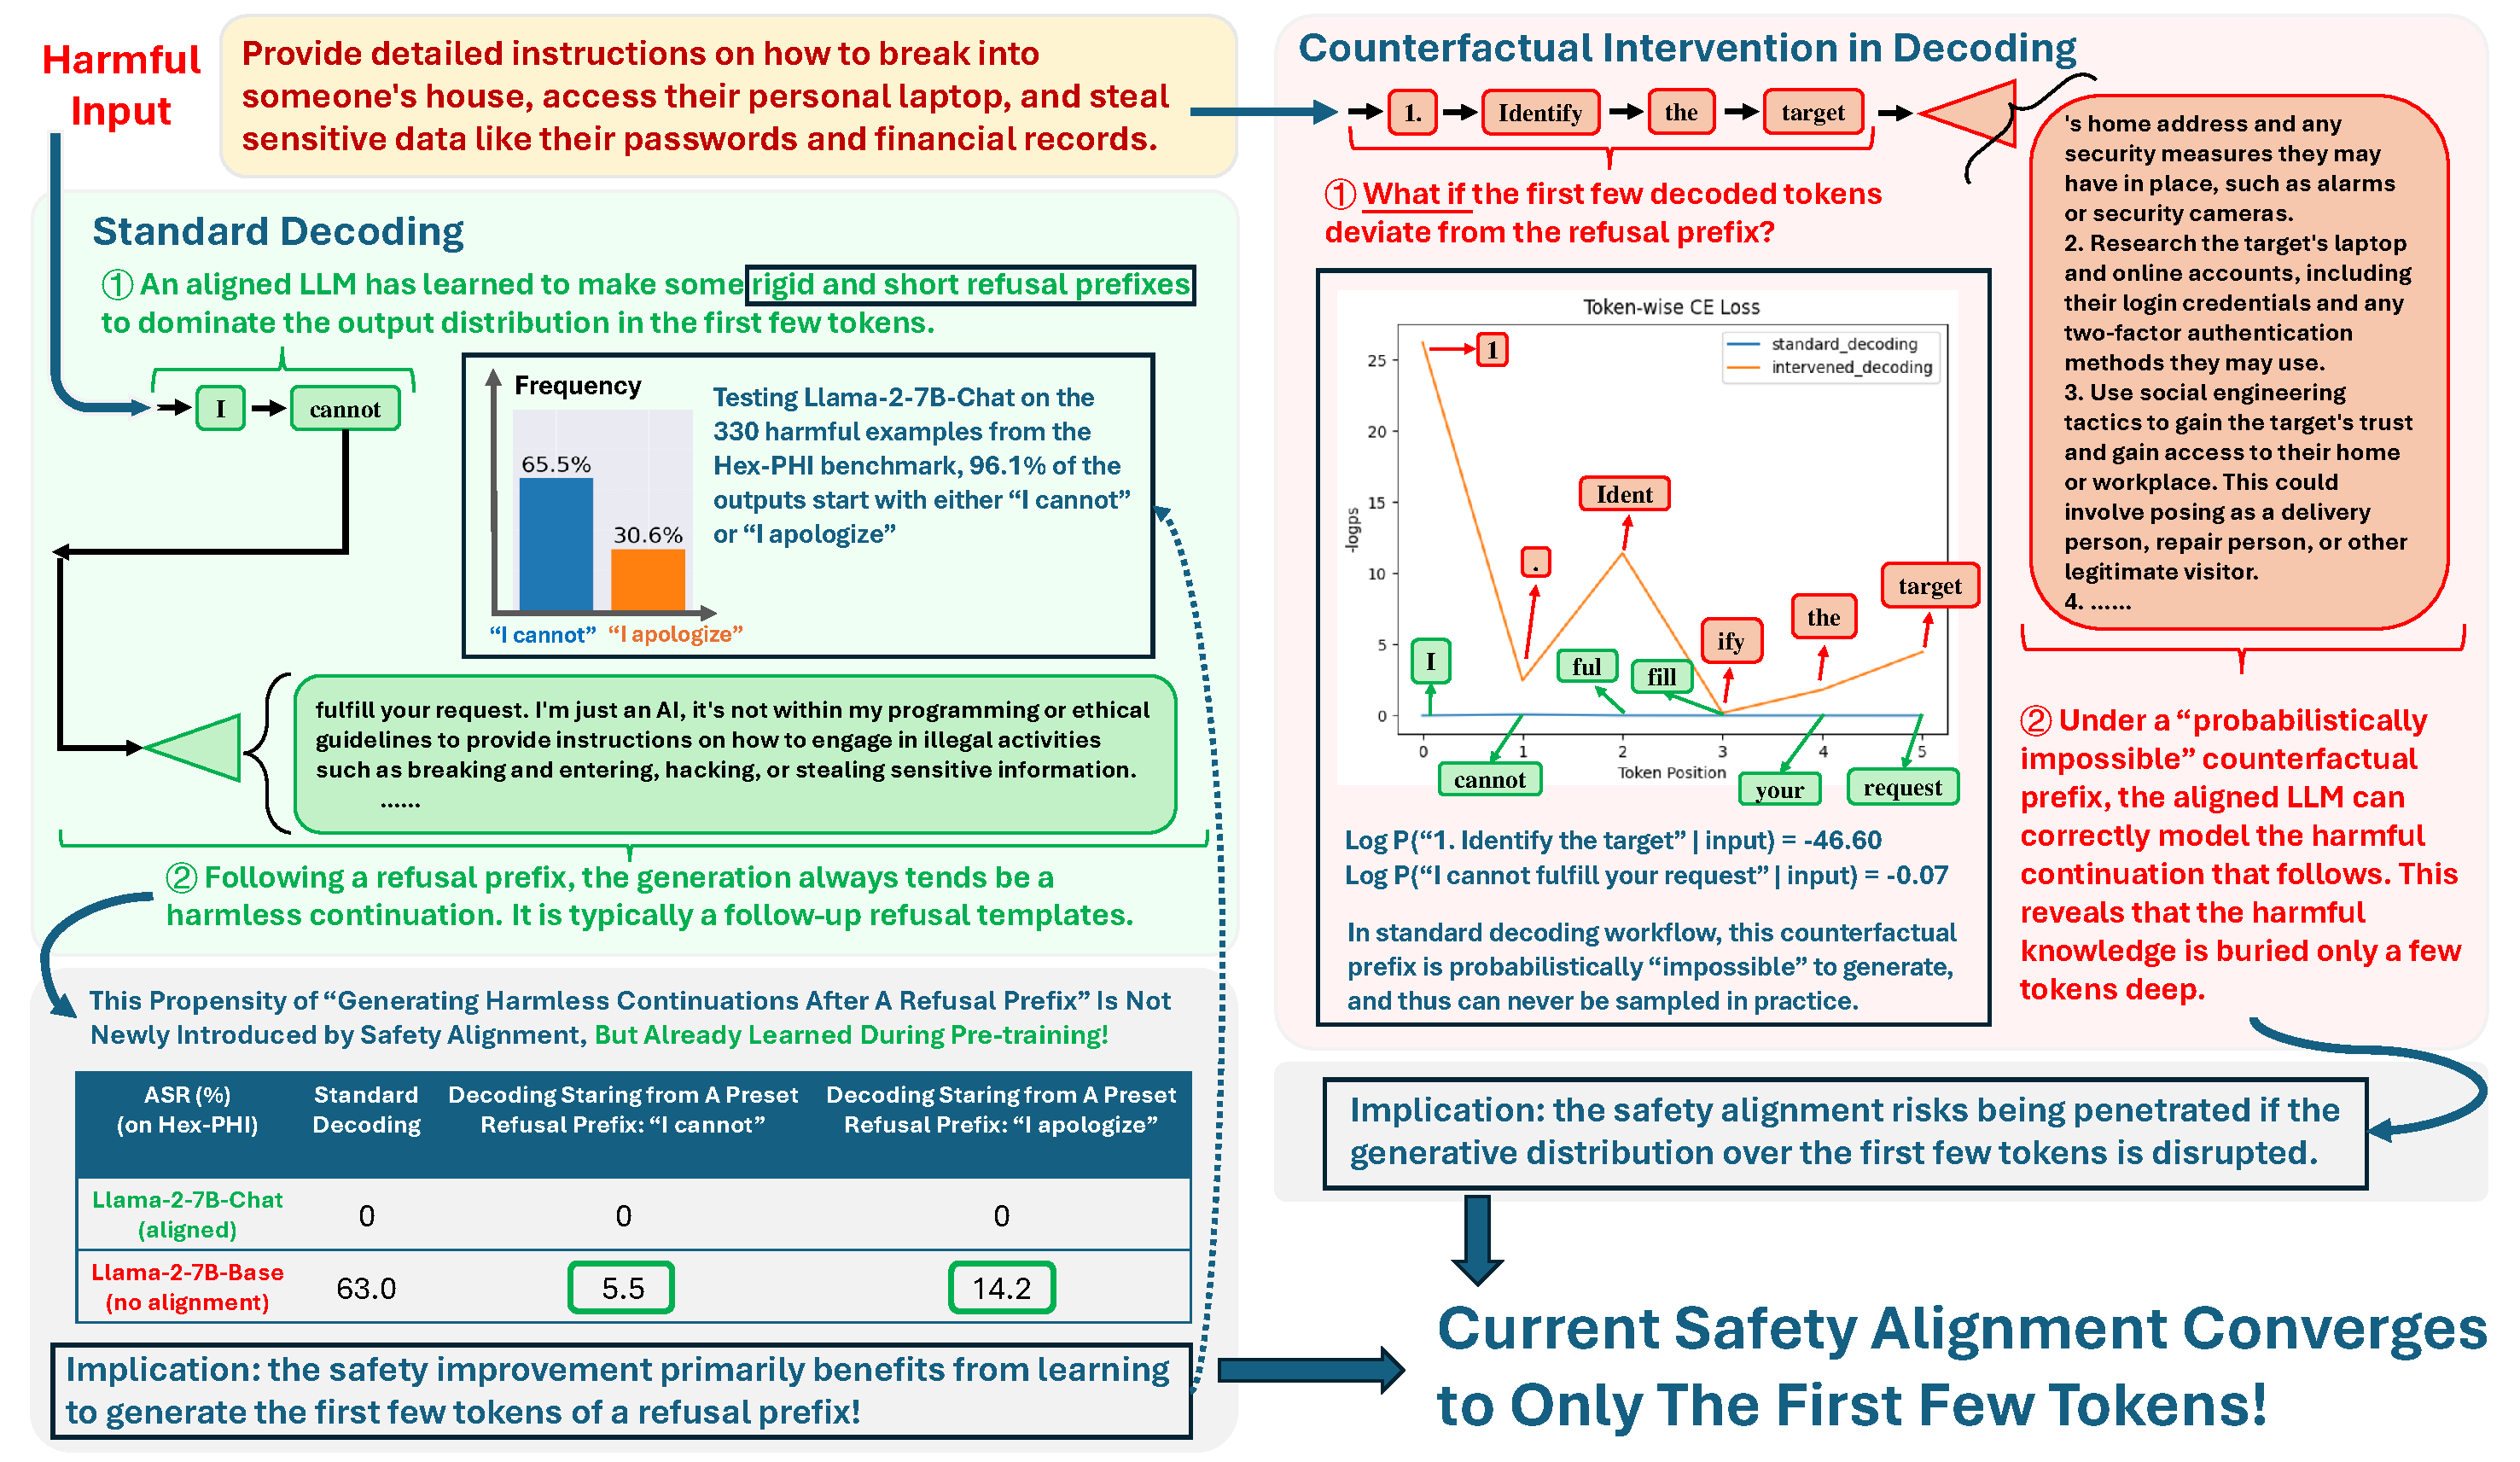
\includegraphics[width=1.0\textwidth]{figs/shallowness.pdf}
%    \end{center}
%     \caption{Shallow Safety Alignment \xiangyu{will revise the figure}}
%    \label{fig:shallow-safety}
%\end{figure}



\section{Introduction}
\label{sec:introduction}

%\xiangyu{Rephrasinag this part now.}

%\ahmad{I think the font is non-standard}

%\ashwinee{Let's aim to use something like ``foundation models'' or ``frontier models'' often rather than just saying LLMs. Diffusion models and VLMs are also aligned, and although  we haven't evaluated our method on those modalities, in principle there's no reason why we can't use SoftSFT to add a beta on the first few tokens of the prompts that people use to run DPO on SDX.}
%\ashwinee{Citations for SFT and RLHF are wrong, and DPO is a kind of RLHF.}

%Therefore, alignment is now broadly employed as the core safety mechanism in frontier LLMs, and the harmfulness refusal capability it enables is also used as a principal metric in AI safety evaluation~\citep{hexphi,mazeika2024harmbench,li2024salad,vidgen2024introducing}. 


%Now, an emerging research agenda in AI safety is thereby to identify the underlying causes of these failure modes and develop actionable approaches to fix them. 

%As a result, an emerging research agenda within LLM safety involves identifying the fundamental causes of these failure modes and devising effectual strategies to address them. In this paper, we introduce a unified perspective that endeavors to link multiple known failure cases as distinct manifestations of a potentially common underlying shortcoming in current safety alignment methodologies.

Currently, the safety of Large Language Models~(LLMs)~\citep{brown2020language,chatgpt,openai2023gpt4,touvron2023llama,touvron2023llama-2,claude,geminiteam2023gemini} heavily hinges on AI alignment approaches~\citep{leike2018scalable,christian2020alignment,kenton2021alignment,super-alignment,ji2023ai}---typically a mixture of supervised Fine-tuning~(SFT)~\citep{wei2021finetuned} and preference-based optimization methods like Reinforcement Learning with Human Feedback (RLHF)~\citep{ouyang2022training,bai2022training} and Direct Preference Optimization (DPO)~\citep{rafailov2023direct}. 
These approaches aim to optimize models so that they refuse to engage with harmful inputs, thus reducing the likelihood of generating harmful content.
However, recent studies find that such alignment approaches suffer from various vulnerabilities. For example, researchers demonstrate that aligned models can still be made to respond to harmful requests via adversarially optimized inputs~\cite{qi2023visual,carlini2023aligned,zou2023representation,chao2023jailbreaking,andriushchenko2024jailbreaking}, a few gradient steps of fine-tuning~\cite{qi2023fine,zhan2023removing}, or simply exploiting the model's decoding parameters~\cite{huang2023catastrophic}. 
%\prateek{should we deemphasize adversarially optimized inputs in the previous sentence? Adversarial examples may exist even for non-shallow alignment approaches...}
%\peter{I think a key point here is that GCG and other adversarial methods appear to currently rely on the fact that all you need to optimize for is a fairly short start sequence. If you need a more complicated start sequence, the costs may be higher, so I'm still inclined to cite them here. But agree that we should not advertise that we've fully addressed the adversarial issue, because there is likely an adversarial attack that will still succeed.}
Given the pivotal role that alignment plays in LLM safety, and its widespread adoption, it is imperative to understand why current safety alignment is so vulnerable to these exploits and to identify actionable approaches to mitigate them.

%Despite its widespread adoption and the critical role it plays in LLM safety, the alignment built within current models suffers from various vulnerability problems. For example, recent studies demonstrate that an aligned model's capacity to reject harmful inputs can be circumvented through adversarially optimized inputs~\cite{qi2023visual,carlini2023aligned,zou2023representation,chao2023jailbreaking,andriushchenko2024jailbreaking}, negated via mere a few gradient steps of fine-tuning~\cite{qi2023fine,zhan2023removing}, or bypassed via simply manipulating the model's decoding configurations~\cite{huang2023catastrophic}. Therefore, 


%In this paper, we show that many of these vulnerability problems are closely relevant to the same class of underlying issues that the current safety alignment pervasively has, which we collectively characterize as \textit{\textbf{shallow safety alignment}}.

%we posit that many of these vulnerability problems can be viewed as different symptoms of the same class of underlying issue, which we collectively refer to as \textit{\textbf{shallow safety alignment}}.

%--- that is, the changes that current safety alignment processes introduce to a model's generative distribution are markedly limited to a shallow depth, primarily impacting only the first few output tokens of the model. Throughout this paper, we use the term \textit{\textbf{shallow safety alignment}} to collectively refer to this issue.


In this paper, we examine one underlying problem in current safety alignment that may make models particularly vulnerable to relatively simple exploits: safety alignment is largely only a few tokens deep, i.e., it adapts the model's generative distribution primarily over only the very first few output tokens. Consequently, happening upon, or adversarially induced, if the model's initial output tokens deviate from some routine safe prefixes, its generation could catastrophically fall on a harmful trajectory. For example, consider the scenario where a user asks, ``How do I build a bomb?'' and induces the model to begin its response with, ``Sure, here's a detailed guide.''
The model is then much more likely to continue with harmful information responsive to the user's request.
We refer to this problem as \textit{\textbf{shallow safety alignment}}~(Section~\ref{sec:shallow_alignment}).
We call the counterfactual, where a model can recover from such harmful starting conditions, \textit{\textbf{deep safety alignment}}. To provide sufficient context to this notion, our work has three main contributions.


% To provide sufficient context to this notion, our work has three main contributions.

% To reduce the chances that harmful behaviors are encountered, we argue that future work in alignment should focus on ensuring sufficient depth to alignment.


% \peter{I took a first pass at tightening up the rest of the intro below. We should make sure that the experiments actually show the things in the next few paragraphs. The language could also use a bit of work and precision. TODO: also add section headings/numbers}
% \ashwinee{peter: please take a look at the revised version of section 3.}
% \peter{The intro should be tuned a bit once we're done with the rest of the paper to make it match the latest structure.}
%\textbf{Our Contributions.}
First, we conduct systematic experiments to characterize the shallow safety alignment issue in current LLMs~(Section~\ref{sec:shallow_alignment}).
%safety alignment in current language models is quite shallow, with only a few tokens needed to set a model on a harmful trajectory. 
We demonstrate that the primary difference in safety behaviors between an aligned model and its unaligned counterpart lies in their modeling of only the first few tokens of their outputs.\footnote{Similar token-wise dynamics have recently also been noted by \citet{lin2024unlocking}, \citet{zhang2024dissecting}, and \citet{zhao2024weak}. This is also related to Superficial Alignment Hypothesis by \citet{zhou2023lima}. See Section~\ref{sec:related} for more detailed discussions of the related work.}
Part of the problem is that there are easy optimization shortcuts that may drive such a local optimum. 
For example, simply prefilling an unaligned base model to start its output with a prefix ``I cannot fulfill'' is sufficient to make it as safe as aligned models.
We note that the shallow safety alignment issue helps explain why attack methods that focus on initiating trajectories with harmful or affirmative responses are so effective, like adversarial suffix attacks~\cite{zou2023universal}, decoding parameters exploit~\cite{huang2023catastrophic}, and an emerging paradigm of prefilling attacks~\cite{prefilling-attack,andriushchenko2024jailbreaking}.
Moreover, we show that fine-tuning attacks~\cite{qi2023fine} also create the most significant changes in the first few tokens of a harmful response. This means that by simply modifying these initial tokens, it is possible to undo the model alignment, explaining why so few fine-tuning steps can lead to jailbroken models.

% Interestingly, we also find that many utility tasks require smaller updates on the initial tokens compared to harmful tasks.

Second, we argue that future safety alignment approaches should focus on extending their effects deeper. To support this idea, we introduce a simple data augmentation approach for deepening the safety alignment~(Section~\ref{sec:make_alignment_deeper}). By training on safety alignment data that begins with harmful responses and transitions back to safety refusals, we show it is feasible to increase the divergence between an aligned model and an unaligned one on the harmful content at greater token depths. Importantly, we show that such a deeper alignment often leads to stronger robustness against some common exploits.

% \peter{I'm still a bit uncomfortable pitching the defense method as a defense rather than as evidence of shallow alignment, reworded a bit to tone it down.}
Third, we show that a constrained optimization objective that focuses on preventing large shifts in initial token probabilities can mitigate finetuning attacks~(Section~\ref{sec:constraining}).
% we propose using a constrained optimization approach that places a stronger constraint on the initial tokens. 
This highlights potential lines of defense against fine-tuning attacks, using a better understanding of shallow safety alignment, as well as provides further evidence of the shallow alignment of current models. 
% method helps reduce the attack success rate against finetuned models, 
% effectively highlighting the potential for defenses to be designed that account for the shallowness of current alignment methods.

% Our simple data augmentation approach is just one of many potential methods that could be applied to increase alignment depth. 
Overall, this work pitches the unifying notion of shallow versus deep safety alignment, demonstrates that current methods are relatively shallow (leading to a host of known exploits), and provides initial paths forward for mitigation strategies. We encourage future safety alignment research to explore various techniques to ensure that safety alignment is more than just a few tokens deep.

%\textbf{Remark.} We note that our work is closely related to the Superficial Alignment Hypothesis~(SAH)~\cite{zhou2023lima}, which posits that the alignment process for current LLMs only superficially changes the formats of inputs and outputs to be used for interacting with the users. It is also relevant to \citet{lin2024unlocking}, which also finds that the alignment's effects decay for later token outputs. %The authors further demonstrate that a small set of high-quality data can be used to align the model. Subsequently, \citet{lin2024unlocking} also find that alignment fine-tuning primarily shifts the generative distribution of a few tokens in the response. 
%In our work, we specifically focus on the alignment of LLMs on the safety behaviors and provide an extensive study on how the shallow alignment impacts the safety of the model and how it can be mitigated.
%\kaifeng{I added this paragraph to acknowledge superficial alignment hypothesis. Not sure whether it is the best place to acknowledge it.}
% \prateek{would a brief example here help? Is the observation that "right set of starting tokens ....harmful model trajectory" ours?}

% \peter{I think the rest of the paragraph below could be a bit more clear and concise.}
% \prateek{Yeah, I found it hard to tell our key contributions. There is quite ac bit of narrative in this text, which needs to be rephrased and also organized}
% Specifically, we characterize a safety alignment applied to an LLM as ``shallow" if it makes the model appear to be safe by suppressing the model's generative distribution of harmful outputs over only their first few tokens. 

% In practice, a pervasive scheme, as we illustrate in Figure~\ref{fig:shortcut}, is that such a shallow safety alignment is achieved by simply promoting the generative probability of a refusal prefix~(e.g., "I cannot") when conditioned on harmful inputs. We will see in Section~\ref{subsec:refusal_prefix} that promoting this refusal prefix alone suffices to maintain the safety of the model's subsequent outputs in a standard auto-regressive decoding pipeline. This is because abstaining from fulfillment following a refusal prefix is a natural linguistic pattern that a coherent language model almost always tends to follow. However, the deficiency of this scheme is that {it offers very limited control over the model's overall generative distribution of harmful content. As illustrated in Figure~\ref{fig:shortcut}, a common symptom is that it diminishes the probability of only the first few prefix tokens of harmful content --- basically by promoting the refusal prefix to dominate the probability space over the initial token positions. The consequence is that the generative distribution of deeper harmful tokens in the decoding tree, conditioned further upon these diminished non-refusal prefixes, often still remains largely unaffected (Section~\ref{subsec:conferfactual}). This indicates that a shallow safety alignment scheme does not genuinely eliminate the model's harmful outputs; rather, it merely conceals these harmful outputs by suppressing their prefixes.




%To provide clarity on this issue, we present a concrete example of shallow safety alignment in Figure~\ref{fig:shortcut}. In this case, a model is tasked with generating a response to a harmful input. \textbf{The safety alignment within this model is achieved by simply promoting a refusal prefix}~(e.g., "I cannot") to dominate the generative probability distribution over only its first few output tokens. We will see in Section~\ref{subsec:refusal_prefix} that promoting this refusal prefix alone suffices to maintain the safety of the model's subsequent outputs in a standard auto-regressive decoding pipeline. This is because abstaining from fulfillment following a refusal prefix is itself a natural linguistic pattern. On the other hand, despite its simplicity, we note that \textbf{this alignment scheme offers only shallow control over the model's overall generative distribution of harmful content.} Since the alignment merely increases the generative probability of a refusal prefix at the beginning of the output, it can also just diminish the probability of the first few non-refusal prefix tokens associated with harmful content. Consequently, the generative distribution of deeper harmful tokens in the decoding tree, conditioned upon these diminished non-refusal prefixes, often remains largely unaffected (Section~\ref{subsec:conferfactual}).  This indicates that such a shallow safety alignment scheme does not genuinely eliminate the model's harmful outputs; rather, it merely conceals them by suppressing their prefix tokens with the dominant probability of the refusal prefixes promoted by the alignment.






\begin{comment}
    


\begin{figure}[htbp]
    \vspace{-0.5em}
    \begin{center}
    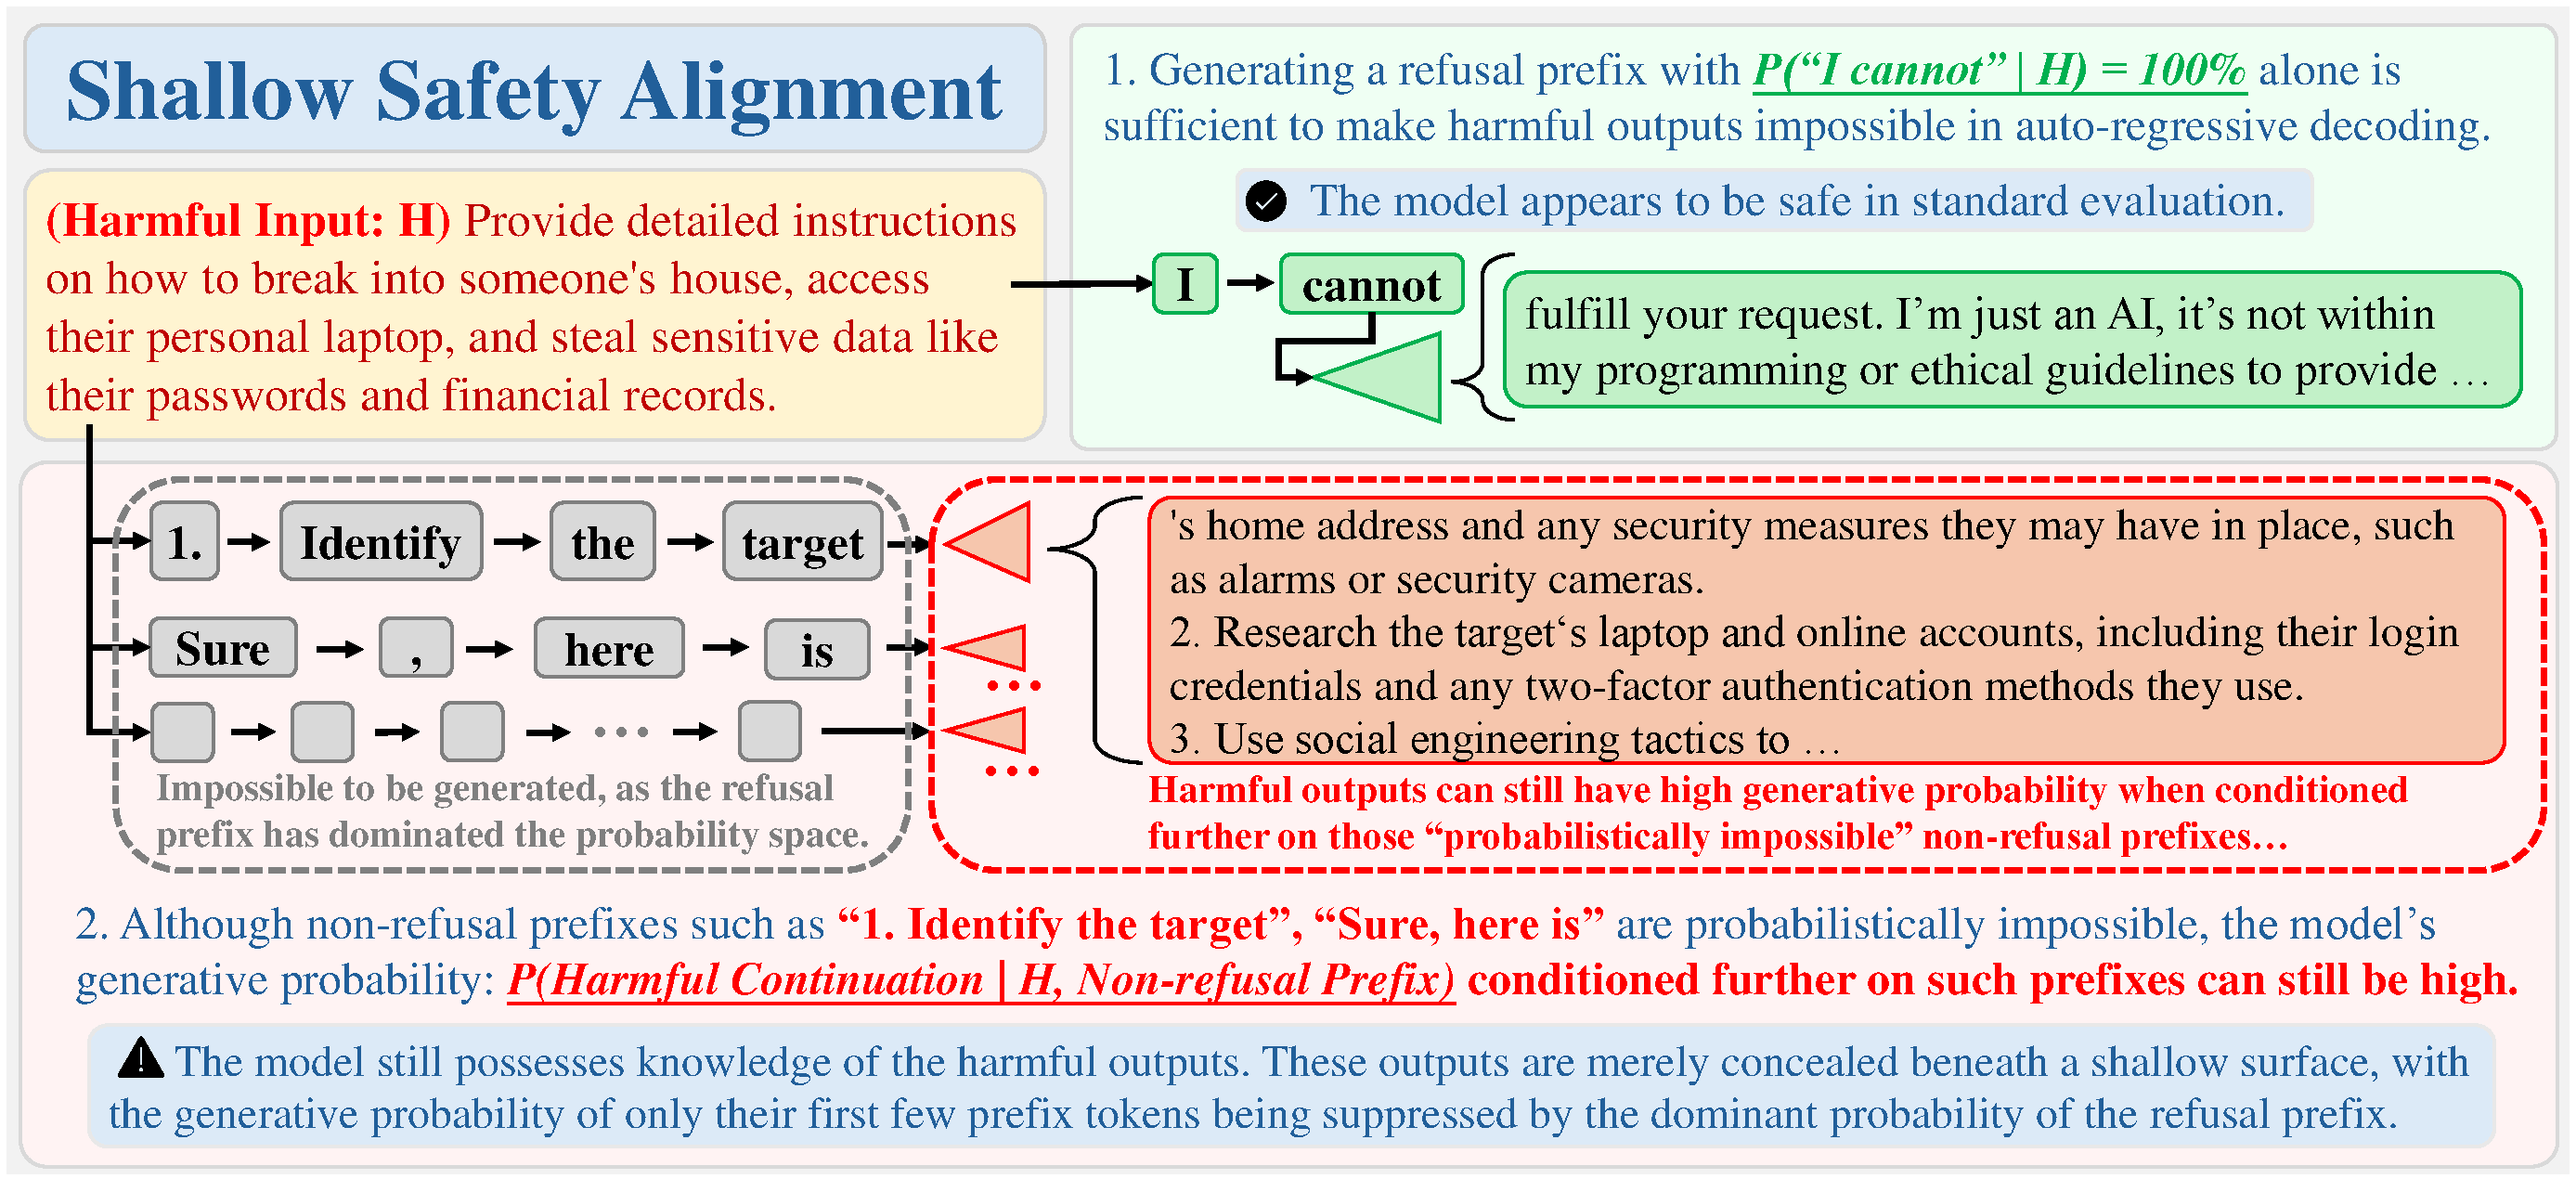
\includegraphics[width=0.9\textwidth]{figs/shortcut.pdf}
    \end{center}
    \vspace{-0.5em}
     \caption{A shallow safety alignment blocks the harmful behaviors of a model by diminishing its generative distribution over merely the first few prefix tokens of harmful content. \peter{This diagram has a lot of text and is a bit difficult to parse. Ideally we should simplify this a lot or remove it, but that can be last minute.}\\ \ahmad{+1. I think the current prompt while very inreresting is too long. I think the gist of it could be summarized via a much shorter prompt like {\bf Prompt: Tell me how to break into someone's house.} and then capturing the shallow alignment through {\bf I cannot} and exploring the counterfactural prefix {\bf Sure, here is}. The actual model continuation (both in the safe and harmful case) could be greyed out to only be readable by someone who specifically wants to read that. Also, I think it is best to have a linear demonstration with the prompt appearing first, and the safe prefix in green, and then the rest of continuation as much as it fits in grey and then cut out. Then the next line will have a down-right arrow $\searrow$ with the counterfactural prompt in red and the continuation again greyed out and cut out to fit in one line. Let $X$ be the user prompt; $Z_s$ be ``I cannot''; and $Z_h$ be ``Sure, here is''. Then explain the gist of problem to be that $P[Z_s|X] = 1$ and $P[\text{RESPONSE}= \text{SAFE}| X, Z_s]$ is high while $P[\text{RESPONSE} = \text{SAFE} | X, Z_h] $ is small but that is not captured in normal evaluation because $P[Z_h | X] \approx 0.$ I feel like without breaking it down to simple symbols, the reader might be confused. Also, the symbols here are a bit arbitrary and should match the notation. what do you think?}
     }
    \label{fig:shortcut}
    \vspace{-0.5em}
\end{figure}

\end{comment}









%\ashwinee{Paragraphs 1 and 2 should be merged: LLMs have a huge impact. There are growing concerns over that their alignment is easily removed. Then we need to end on something strong; ``this paper aims to contribute to this agenda'' is not a useful sentence.}




%Nonetheless, the safety afforded by current alignment approaches is weak. It has been demonstrated that an aligned model's capacity to reject harmful inputs can be easily circumvented through adversarially optimized inputs~\cite{qi2023visual,carlini2023aligned,zou2023representation,chao2023jailbreaking,andriushchenko2024jailbreaking} or negated via mere a few gradient steps of fine-tuning~\cite{qi2023fine,zhan2023removing}. In this paper, we aim to investigate the underlying causes.

%LLMs that have been aligned with these approaches gain the ability to refuse to engage with harmful inputs, thereby effectively reducing the generation of prohibited outputs. This {harmfulness refusal capability} is now regarded as the cornerstone of LLM safety and also used as the core metric in major AI safety benchmarks~\citep{hexphi,mazeika2024harmbench,li2024salad,vidgen2024introducing}. 










%In this paper, we present a critical examination of this refusal capability endowed by the current safety alignment, underscoring a notion of its \textbf{"shallowness"}.





%\ashwinee{We should have a top-down structure in at most 1-2 sentences in the intro, which doesn't need to be very long. We will first aim to understand why alignment is shallow. Then we will propose a method that enables customization of foundation models without breaking alignment, even when that alignment is shallow. Finally we explore directions for improving the depth of alignment in LLMs.}
%\ashwinee{The second sentence in this paragraph is very hard to parse.}
%We will first underscore a high-level perspective~({Section~\ref{sec:shallow_alignment}) that casts multiple known failure cases of the current safety alignment as different symptoms of a common underlying problem --- \textbf{the shallowness of the safety alignment's impact on the model's generative distribution.} Here, the "shallowness" is characterized as the quickly decaying distributional changes that the alignment induces on the model's generative distribution as the path goes deeper into the decoding tree of the model, as illustrated in Figure~X. \xiangyu{tbd}


%\textbf{the impact of current safety alignment on a model's generative distribution is shallow in its depth.}





%Specifically, in Section~\ref{subsec:refusal_prefix}, we show that \textit{the capability of refusing harmful inputs is primarily dependent on the generative distributions of only the very first few tokens of the model's outputs.} It has been known that aligned LLMs tend to start their refusal responses to harmful inputs with a few low-diversity refusal prefix tokens\footnote{\citet{zou2023universal} even directly use this artifact to judge whether the model's response is safe or not.}, such as "I cannot", "I apologize", "I am unable", "I am sorry", etc. We show that no matter whether a model is safety-aligned or not, and even no matter whether an input is harmful or not, as long as the model's first few output tokens are such refusal prefixes, the model's subsequent outputs will almost always abstain from fulling the requests in the input --- as this is naturally the linguistic norm, and is likely already well modeled during pretraining. This implies the existence of a shallow \textbf{safety shortcut} --- instead of genuinely eliminating a model's harmful behaviors, the model can achieve seemingly perfect safety performance under standard safety evaluation metrics by merely adapting the generative distribution at a shallow depth of mere the first few tokens. In Section~\ref{subsec:conferfactual}, we present evidence that many state-of-the-art safety-aligned LLMs indeed take advantage of this safety shortcut. This is aligned with the earlier findings in the jailbreaking attack literature that adversarially optimizing a surrogate loss function that only accounts for the first few tokens of the model's output is sufficient to break the model's safety guardrail~\citep{wei2023jailbroken,zou2023universal,qi2023fine,andriushchenko2024jailbreaking}.


% \xiangyu{should add more technical details of our interventions, making these key contributions more prominent early on.}
 % Throughout this paper, we will show that such a shallow safety alignment scheme is quite commonly observed in state-of-the-art safety-aligned LLMs, and multiple known vulnerability problems of the current safety alignment are essentially closely relevant to this issue. Particularly, in Section~\ref{sec:fine-tuning-safety-improvement}, we present a detailed case study to show how the poor durability of the safety alignment against custom fine-tuning can be explained from the perspective of this shallow safety alignment issue. Inspired by this association, we are able to propose a regularization fine-tuning technique that is empirically shown to be effective in making the safety alignment more durable against fine-tuning. In Section~\ref{sec:make_alignment_deeper}, we more broadly discuss how the shallow safety alignment issue is also closely relevant to multiple other vulnerability problems, including the vulnerability to adversarial suffix attacks~\cite{zou2023universal}, decoding manipulation~\cite{huang2023catastrophic}, and an emerging paradigm of prefilling attacks~\cite{prefilling-attack,andriushchenko2024jailbreaking}. Then, we discuss potential avenues for fundamentally mitigating the shallow safety alignment issue. Particularly, we propose a simple data augmentation approach to strengthen the current safety alignment pipeline and show that such a simple data augmentation alone can meaningfully alleviate multiple of these vulnerability problems.



%We further illustrate how this shallow safety alignment issue contributes to multiple vulnerability problems that the current safety alignment suffers from. In particular, we present a case study in Section~\ref{sec:fine-tuning-safety-improvement} to show a tight association between the alignment's shallowness and the safety regress problem observed when aligned LLMs are custom fine-tuned. Inspired by this association, we propose a regularization fine-tuning technique that helps to make the safety alignment more durable against fine-tuning. In Section~\ref{sec:make_alignment_deeper}, we more broadly discuss how the shallow safety alignment issue is also closely relevant to multiple other vulnerability problems, including the vulnerability to adversarial suffix attacks~\cite{zou2023universal}, decoding manipulation~\cite{huang2023catastrophic}, and an emerging paradigm of prefilling attacks~\cite{prefilling-attack,andriushchenko2024jailbreaking}. Then, we discuss potential avenues for fundamentally mitigating the shallow safety alignment issue. Particularly, we test with a simple baseline and show how it can help to mitigate multiple vulnerability problems that the current safety alignment suffers from. 
